\documentclass[AutoFakeBold,AutoFakeSlant]{beamer}
\usepackage{ctex}
\usepackage{hyperref}
\usepackage[defaultsans]{droidsans}
\usepackage{fontspec}
\usepackage{newtxmath}
\usepackage{latexsym,amsmath,xcolor,multicol,booktabs,calligra,tcolorbox}
\usepackage{graphicx,tabularx,multirow,makecell}
\usepackage{listings}
\lstset{
    basicstyle=\ttfamily\tiny,
    breaklines=true,
    breakatwhitespace=true,
    columns=fullflexible,
    frame=single,
    backgroundcolor=\color{gray!6},
}
\usepackage{tikz}
\usetikzlibrary{arrows.meta,positioning}

\usetheme{Madrid}
\usecolortheme{default}
\setbeamertemplate{navigation symbols}{}
\setbeamertemplate{footline}[frame number]

\graphicspath{{./figures/}}
% 与本次流水线输出目录一致：跑完 pipeline 后把此处改成你的 pipeline_<时间戳>
\newcommand{\PipelineOutName}{pipeline\_20260406\_201540}

\author{李禹江，张博涵，蒋兴宇}
\title{隐私政策切句与个信法相关句筛选}
\subtitle{\texorpdfstring{Lab\,2-3：Data Safety 衔接与 WEEK\_4 流水线实验汇报}{Lab 2-3 Data Safety 与 WEEK4 流水线汇报}}
\institute{我的刀盾队}
\date{\today}

\begin{document}
\kaishu

\begin{frame}
    \titlepage
\end{frame}

\begin{frame}
    \frametitle{目录}
    \tableofcontents
\end{frame}

\section{实验目标}

\begin{frame}
    \frametitle{实验目标（对齐课程讲义 Lab\,2-3）}
    \begin{itemize}
        \item 将各应用隐私政策\textbf{切分为句子}，保留 \texttt{doc\_id}、\texttt{sent\_index}，便于回溯原文位置。
        \item 对每句做\textbf{二分类}：是否与\textbf{个人信息的处理与利用}相关（收集、使用、存储、共享、跨境、安全、权利响应等）。
        \item 输出 \texttt{sentences.jsonl}、\texttt{stats.json} 及与 WEEK\_3 \texttt{2-2} 同列的 \texttt{sentences\_week3\_2\_2.csv}，服务后续\textbf{人工抽检}与 \texttt{run\_audit} 衔接。
        \item 附带\textbf{关键词弱信号} \texttt{keyword\_hint}，用于粗排序与对照，\textbf{不替代}模型结论。
    \end{itemize}
\end{frame}

\section{实验环境}

\begin{frame}
    \frametitle{实验环境}
    \begin{itemize}
        \item \textbf{操作系统}：Windows 10/11；Shell：PowerShell。
        \item \textbf{Python}：3.10+）。
        \item \textbf{核心依赖}：\texttt{pandas}）、\texttt{matplotlib}、\texttt{ollama}。
    \end{itemize}
\end{frame}

\section{实验过程}

\begin{frame}
    \frametitle{实验流程概览}
    \centering
    \begin{tikzpicture}[
        node distance=6mm and 8mm,
        box/.style={draw, rounded corners, align=center, minimum width=2.6cm, minimum height=8mm, font=\small},
        arr/.style={-{Latex[length=2mm]}, thick},
    ]
        \node[box, fill=blue!8] (raw) {UTF-8 政策文本};
        \node[box, fill=blue!8, right=of raw] (split) {切句\\\texttt{sentence\_split}};
        \node[box, fill=green!12, right=of split] (cls) {LLM 分类\\\texttt{classify}};
        \node[box, fill=orange!15, below=of cls] (out) {JSONL / stats /\\WEEK\_3 CSV};
        \node[box, fill=violet!10, left=of out] (plot) {统计与作图\\\texttt{plot\_experiment}};
        \node[box, fill=gray!12, left=of plot] (audit) {基于隐私相关句子分析应用级审计};
        \draw[arr] (raw) -- (split);
        \draw[arr] (split) -- (cls);
        \draw[arr] (cls) -- (out);
        \draw[arr] (out) -- (plot);
        \draw[arr, dashed] (out) -- (audit);
    \end{tikzpicture}
\end{frame}

\section{实验结果}

\begin{frame}
    \frametitle{五款应用与数据来源}
    \begin{itemize}
        \item \textbf{对象应用}：\textbf{小红书}、\textbf{LOFTER}、\textbf{Blued 极速版}、\textbf{世纪佳缘}、\textbf{Soul}。
        \item \textbf{处理内容}：各应用隐私政策全文 $\rightarrow$ 切句 $\rightarrow$ 句子级「个人信息处理相关」二分类 $+$ 规则 \texttt{keyword\_hint}。
    \end{itemize}
\end{frame}

\begin{frame}
    \frametitle{五款应用分项结果（完整指标）}
    \tiny
    \begin{tabularx}{\textwidth}{|l|r|r|r|r|r|}
        \toprule
        \textbf{应用} & \textbf{总句} & \textbf{相关} & \textbf{无关} & \textbf{模型相关占比} & \textbf{关键词占比} \\
        \midrule
        小红书 & 296 & 230 & 65 & 77.70\% & 55.74\% \\
        LOFTER & 227 & 198 & 29 & 87.22\% & 59.91\% \\
        Blued 极速版 & 192 & 171 & 21 & 89.06\% & 63.54\% \\
        世纪佳缘 & 323 & 286 & 37 & 88.54\% & 63.16\% \\
        Soul & 347 & 293 & 54 & 84.44\% & 66.57\% \\
        \midrule
        \textbf{合计} & \textbf{1385} & — & — & $\approx$\textbf{85.1\%} & — \\
        \bottomrule
    \end{tabularx}
    \scriptsize
    \begin{itemize}
        \item 「模型相关占比」：分应用为 \textbf{相关/总句}；合计为五应用相关句之和除以总句数，即 \textbf{1178/1385}。
    \end{itemize}
\end{frame}

\begin{frame}
    \frametitle{数据规模：五款应用切句数量}
    \begin{columns}
        \begin{column}{0.48\textwidth}
            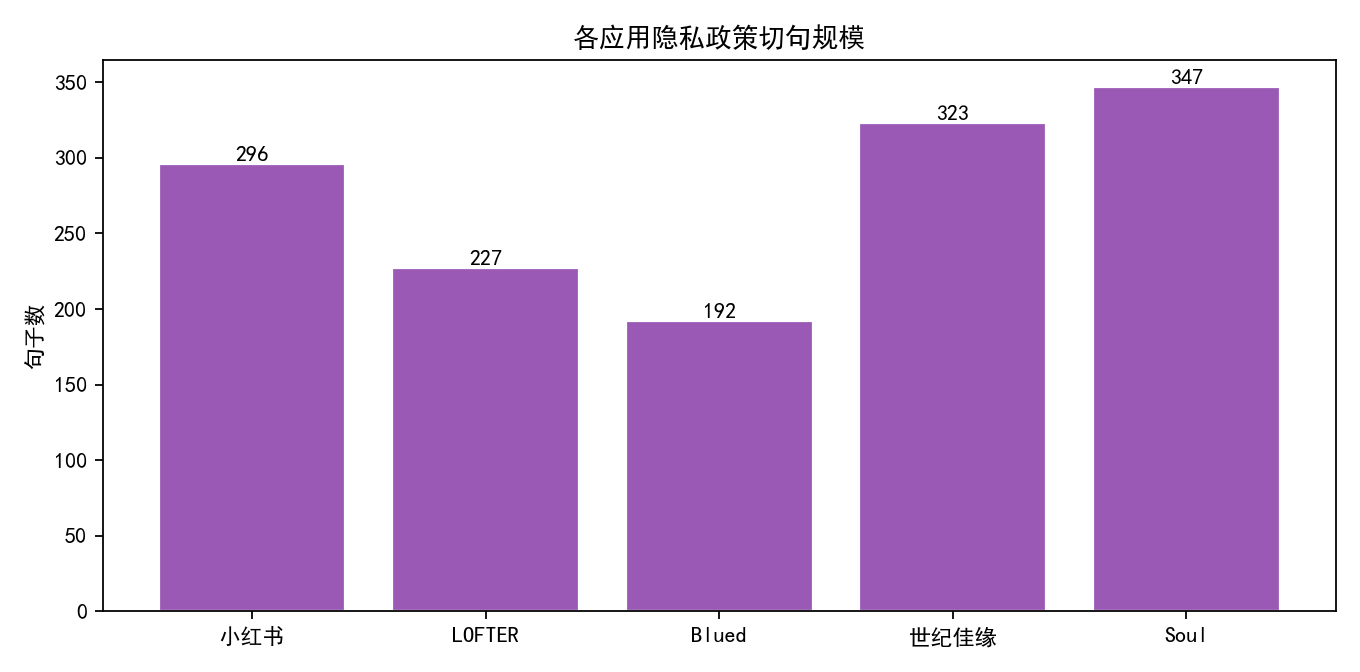
\includegraphics[width=\linewidth]{fig_totals_by_app.png}
        \end{column}
        \begin{column}{0.52\textwidth}
            \small
            \begin{itemize}
                \item 全量流水线共 \textbf{1385} 句。
                \item 规模最大：\textbf{Soul}（347 句）；最小：\textbf{Blued 极速版}（192 句）。
            \end{itemize}
            \vspace{0.3em}
            \begin{tabular}{l r}
                \toprule
                \textbf{应用} & \textbf{句数} \\
                \midrule
                小红书 & 296 \\
                LOFTER & 227 \\
                Blued 极速版 & 192 \\
                世纪佳缘 & 323 \\
                Soul & 347 \\
                \midrule
                \textbf{合计} & \textbf{1385} \\
                \bottomrule
            \end{tabular}
        \end{column}
    \end{columns}
\end{frame}

\begin{frame}[fragile]
    \frametitle{关键词弱信号：\texttt{keyword\_hint} 规则}
    \scriptsize
    对每条句子用正则子串匹配；任一词干出现则 \texttt{keyword\_hint=true}，统计入绿色柱的「命中占比」。
    \vspace{0.35em}
\begin{lstlisting}[language=Python, alsoletter={|}, morekeywords={Pattern}]
_HINT_RE: Pattern[str] = re.compile(
    r"(个人信息|个人敏感信息|隐私|收集|处理|使用|存储|保存|共享|转让|"
    r"披露|委托|跨境|第三方|SDK|权限|设备信息|位置|通讯录|相册|相机|"
    r"麦克风|日志|Cookie|标识符|IMEI|OAID|IDFA|MAC|IP|账号|手机号|"
    r"实名|注销|撤回|删除|更正|复制|查阅|未成年人|儿童|敏感)"
)
\end{lstlisting}
\end{frame}

\begin{frame}
    \frametitle{规则弱信号 vs 模型「个信相关」占比}
    \begin{columns}
        \begin{column}{0.55\textwidth}
            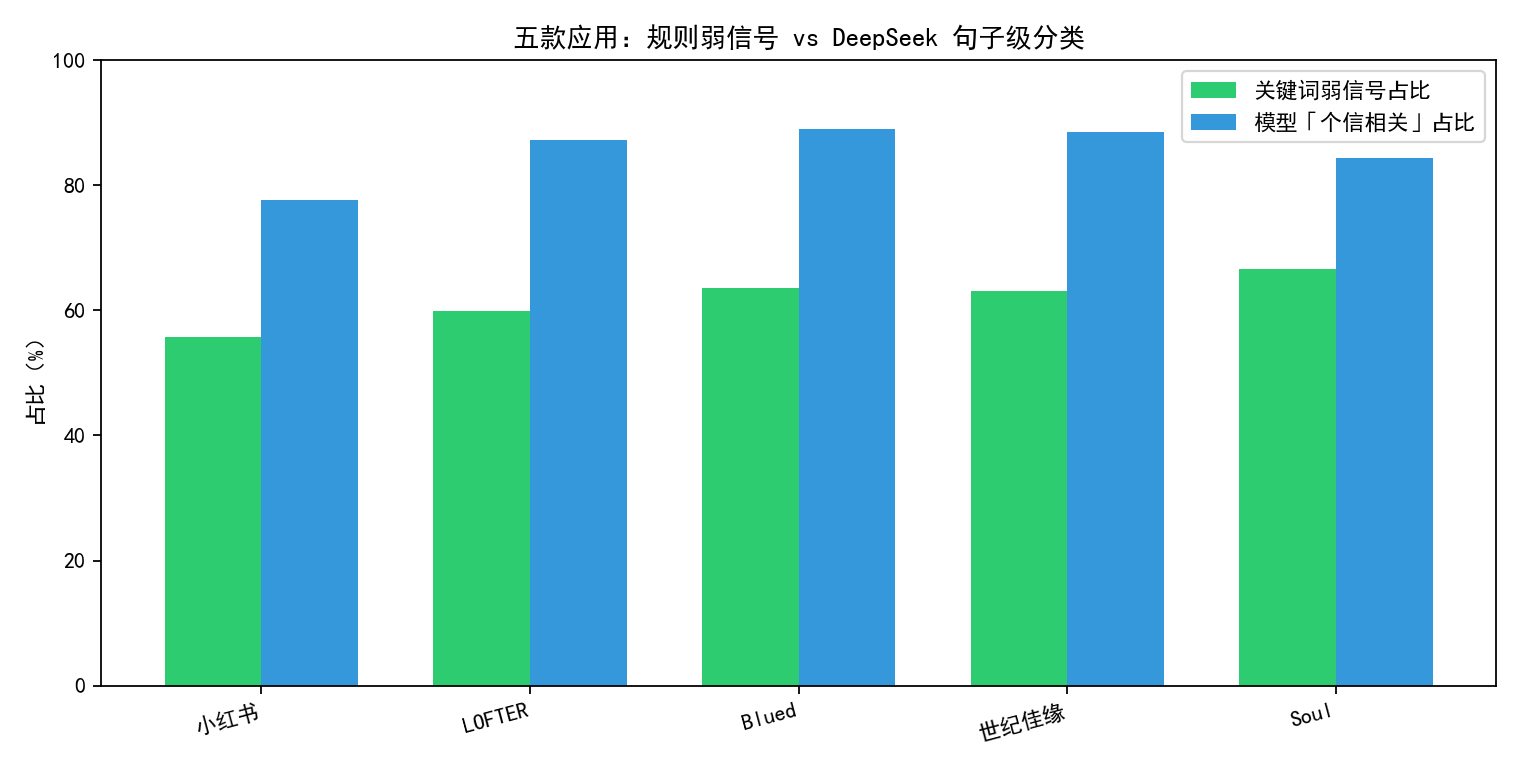
\includegraphics[width=\linewidth]{fig_ratios_by_app.png}
        \end{column}
        \begin{column}{0.45\textwidth}
            \scriptsize
            \begin{itemize}
                \item 绿色柱：\texttt{keyword\_hint} 命中占比（词干正则见「\texttt{keyword\_hint} 规则」帧）；蓝色柱：模型判「相关」占全句比例。
                \item 模型占比\textbf{系统高于}关键词：弱规则无法覆盖全部表述，LLM 可补全「无关键词仍属个信处理」的句子。
                \item 跨应用差异反映政策写法与非隐私段落比例不同，可用于\textbf{分层抽检}。
            \end{itemize}
        \end{column}
    \end{columns}
\end{frame}

\begin{frame}
    \frametitle{模型判「相关」的句数（绝对量）}
    \centering
    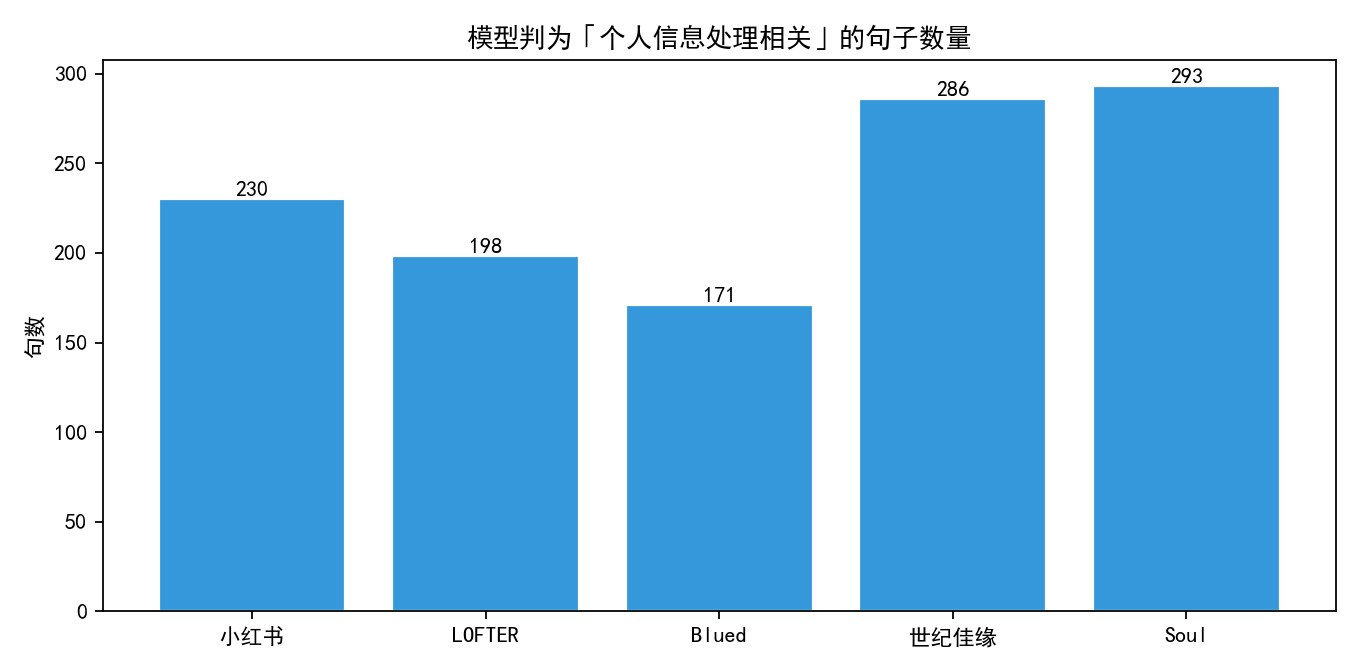
\includegraphics[width=0.88\linewidth]{fig_pii_true_by_app.png}
    \vspace{0.4em}
    \begin{itemize}
        \item 五应用合计：模型判「相关」\textbf{1178} 句，占全量 \textbf{1178/1385 $\approx$ 85.1\%}。
    \end{itemize}
\end{frame}

\begin{frame}
    \frametitle{典型案例：Soul 关键词 / 模型计数与句长分布}
    \begin{columns}
        \begin{column}{0.5\textwidth}
            \centering
            
\includegraphics[width=\linewidth]{soul_detail/stats_counts.png}
        \end{column}
        \begin{column}{0.5\textwidth}
            \centering
            
\includegraphics[width=\linewidth]{soul_detail/sentence_length_hist.png}
        \end{column}
    \end{columns}
    \vspace{0.3em}
    \scriptsize
    左：规则与模型分类句数；右：句长直方图（字符数），用于观察切句粒度与长句抽检需求。
\end{frame}

\begin{frame}
    \frametitle{拓展：句子表 + WEEK\_3 audit 抽样（每应用前 20 行）}
    \centering
    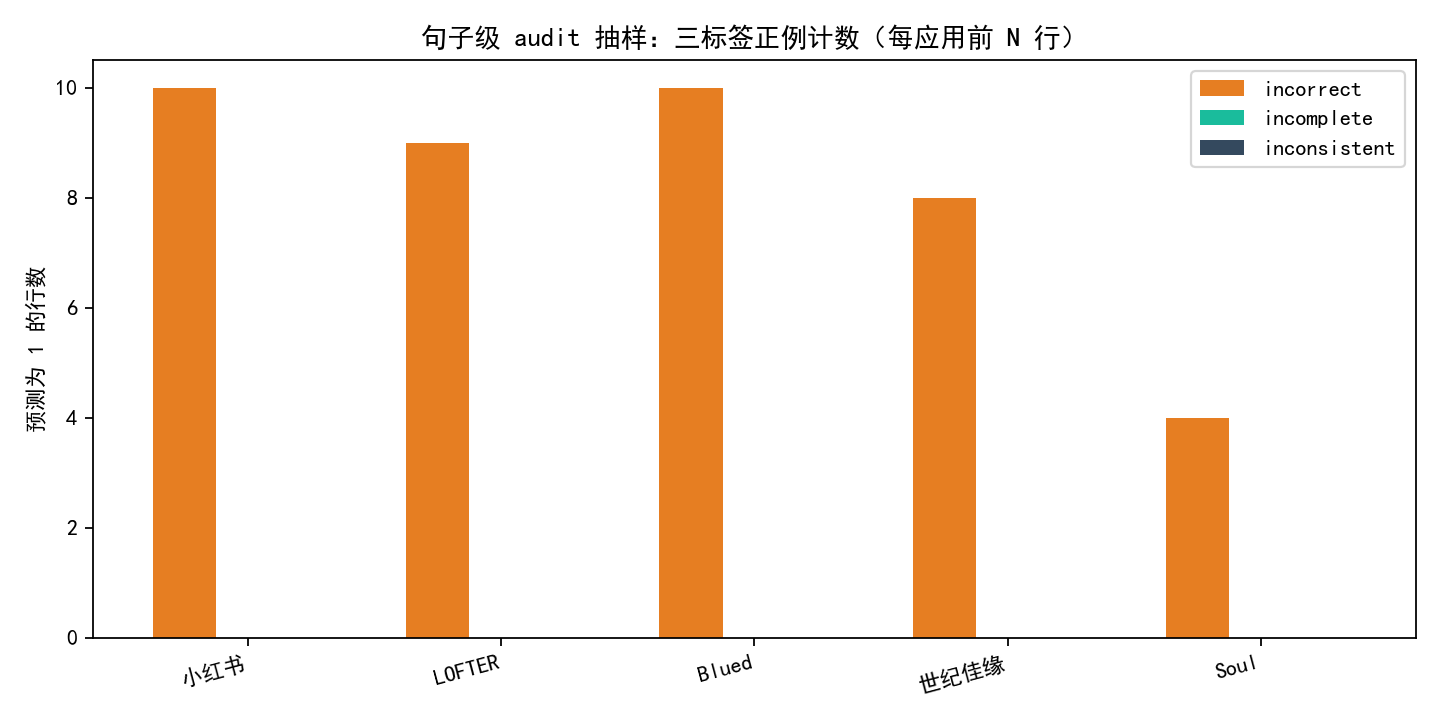
\includegraphics[width=0.92\linewidth]{fig_audit_by_app.png}
    \vspace{0.4em}
    \begin{itemize}
        \item 横轴为各应用，纵轴为预测标签为 1 的行数。
        \item \textbf{注意}：句级 CSV 中 Data Safety 多为占位，与「完整 DS vs 全文 PP」应用级审计不等价，结果仅供流程演示与误例分析。
    \end{itemize}
\end{frame}

\begin{frame}
    \frametitle{指标汇总表（摘自各应用 \texttt{stats.json}）}
    \tiny
    \begin{tabularx}{\textwidth}{|l|r|r|r|}
        \toprule
        \textbf{应用} & \textbf{总句数} & \textbf{模型相关占比} & \textbf{关键词占比} \\
        \midrule
        小红书 & 296 & 77.70\% & 55.74\% \\
        LOFTER & 227 & 87.22\% & 59.91\% \\
        Blued 极速版 & 192 & 89.06\% & 63.54\% \\
        世纪佳缘 & 323 & 88.54\% & 63.16\% \\
        Soul & 347 & 84.44\% & 66.57\% \\
        \bottomrule
    \end{tabularx}
    \vspace{0.5em}
\end{frame}

\section{可能的提升方向}

\begin{frame}
    \frametitle{可能的提升方向}
    \begin{itemize}
        \item \textbf{数据质量}：固定政策版本日期字段，便于合规追溯。
        \item \textbf{提示与模型}：细化边界句定义（法律援引、口号句是否算「相关」）；对比 Qwen/Ollama 本地模型与 DeepSeek，做一致性抽检。
        \item \textbf{弱监督与评测}：分层随机抽样算人工一致率；发布 10--20 条\textbf{标注指南}稳定标签语义。
        \item \textbf{讲义拓展}：对 \texttt{sentences.jsonl} 做句向量 + UMAP/HDBSCAN 聚类，辅助主题分布与难例挖掘（非必做）。
        \item \textbf{工程化}：高价值子集按 \texttt{pii\_related} 与 \texttt{keyword\_hint} 联合排序后送标。
    \end{itemize}
\end{frame}

\begin{frame}
    \begin{center}
        {\Huge 感谢聆听！}
    \end{center}
\end{frame}

\end{document}
